\subsection{Reduction by killing}

Reduction by killing allows us to \emph{clear} (set to $\bm 0$) certain columns throughout the reduction process, allowing us to avoid unnecessary column operations that would lead the column to being zero anyway. This technique was first introduced by \textcite{chen2011persistent}.

We recall that persistent homology aims to track the changes to the homology groups of a chain complex as we move through a filtration. We now formalise how simplices may change the homology groups.

\begin{definition}[Positive and negative simplices]
  Let $\mathbb K = \{K_i\}_{i=0}^n$ be a maximal filtered simplicial complex of a simplicial complex $K$ with induced simplex ordering $\sigma_1, \ldots, \sigma_n$. Let $\iota_i: K_i \xhookrightarrow{} K_{i+1}$ be the inclusion map and $\overline\iota_i: H_*(K_i) \to H_*(K_{i+1})$ the induced map on homology. 
  \begin{enumerate}
    \item $\sigma_i \in K$ is said to be a \emph{positive simplex} if its addition creates a homology class. That is, for all $[c] \in H_*(K_{i-1})$ we have $\overline\iota_{i-1}([c]) \neq [\sigma_i] \in H_*(K_i)$.
    \item $\sigma_i \in K$ is said to be a \emph{negative simplex} if it its addition destroys a homology class. That is, there is $[c], [c'] \in H_*(K_{i-1})$ with $[c] \neq [c']$ such that $\overline\iota_{i-1}([c]) = \overline\iota_{i-1}([c']) = [\sigma] \in H_*(K_i)$.
  \end{enumerate} 
\end{definition}

We can pair each negative simplex $\sigma_j \in K$ with the positive simplex $\sigma_i \in K$ ($i < j$) that created the class that $\sigma_j$ destroys. We call $(i, j)$ (or $(\sigma_i, \sigma_j)$) a \emph{persistence pair}, and $j - i$ its \emph{index persistence}. It is clear (from the definition of homology) that for a persistence pair $(\sigma_i, \sigma_j)$, we have $\dim\sigma_i = \dim\sigma_j - 1$. 

\begin{corollary}\label{lem:positive-or-negative-simplices}
  Let $\mathbb K = \{K_i\}_{i=0}^n$ be a maximal filtered simplicial complex of a simplicial complex $K$. Then every simplex $\sigma \in K$ is either \emph{positive} or \emph{negative}.
\end{corollary}

This is a direct consequence of Lemma \ref{lem:reduction-correct}.

Note that, although each simplex either creates or destroys a homology class, not every simplex belongs to a persistence pair as described above. In particular, certain simplices create homology classes that persist through to the final complex, $K_n = K$. Such (positive) simplices are called \emph{essential simplices}.

The following is the key observation for reduction by killing.

\begin{lemma} \label{lem:clearing-lemma}
  Let $\mathbb K = \{K_i\}_{i=0}^n$ be a maximal filtered simplicial complex of a simplicial complex $K$ with induced simplex ordering $\sigma_1, \ldots, \sigma_n$, let $R$ be the reduction of the boundary matrix of $\mathbb K$ (with respect to our ordering), and let $(i, j) \in \Pers(H_*(\mathbb K))$. Then $R_i = \bm 0$. 
\end{lemma}

\begin{proof}
  As $(i, j) \in \Pers(H_*(\mathbb K))$, $\low_R(j) = i$. Suppose $R_i \neq 0$, then $\low_R(i) = i'$ for some $i \in \{1, \ldots, n\}$. But then $(\sigma_{i'}, \sigma_i)$ is a persistence pair, contradicting Corollary \ref{lem:positive-or-negative-simplices}.
\end{proof}

So if we discover a negative simplex $\sigma$, we can clear the column corresponding to the simplex whose homology class $\sigma$ kills. However, the standard algorithm \textsc{S} starts at the left side of the boundary matrix and moves to the right, so we will always discover positive simplices first. Thus we do not save any column operations. 

To take advantage of Lemma \ref{lem:clearing-lemma}, we instead reduce the boundary matrix right-to-left. We first clear the $d = \dim K$ simplices (from left-to-right), then the $(d-1)$-simplices, and so on. 

Algorithm \ref{alg:reduction-by-killing} shows the modified algorithm, and we denote this speed-up with the sparse matrix representation on top of the standard algorithms as \textsc{SSR}.

\begin{algorithm}
  \caption{The reduction by killing (\textsc{SSR}) algorithm for \textsc{$\mathbb F_2$-\-Pers\-Reduc\-tion}.}
  \label{alg:reduction-by-killing}
  \begin{algorithmic}[1]
      \Function{StdReduction}{$n \times n$ boundary matrix $\partial$}
        \State $R \gets \partial$
        \For{$k \gets d$ to $1$}
          \For{$i \gets 1$ to $n$}
            \If{simplex $i$ does not have dimension $k$}
              \State continue to next simplex
            \EndIf
            \While{not \Call{IsColReduced}{$R, i$}}
              \For{$j=1$ to $i$}
                \If{$\Call{Low}{R, i} = \Call{Low}{R, j}$}
                  \State add column $j$ to $i$ and break for loop
                \EndIf
              \EndFor
            \EndWhile
            \If{$R_j \neq \bm 0$}
              \State clear column $\low(R, j)$
            \EndIf
          \EndFor
        \EndFor
        \State\Return $R$
      \EndFunction
  \end{algorithmic}
\end{algorithm}

An experiment was conducted comparing \textsc{SS} and \textsc{SSR}. A Vietoris-Rips filtration was constructed from a sample of 1000 points from the noisy unit circle (radius fluctuation $\pm 0.05$). We run both algorithms from $\varepsilon = 0.01$ to $\varepsilon = 0.06$. Figure \ref{fig:speedups-2v3-compute} shows the result of this experiment.

\begin{figure}
  \makebox[\textwidth][c]{
    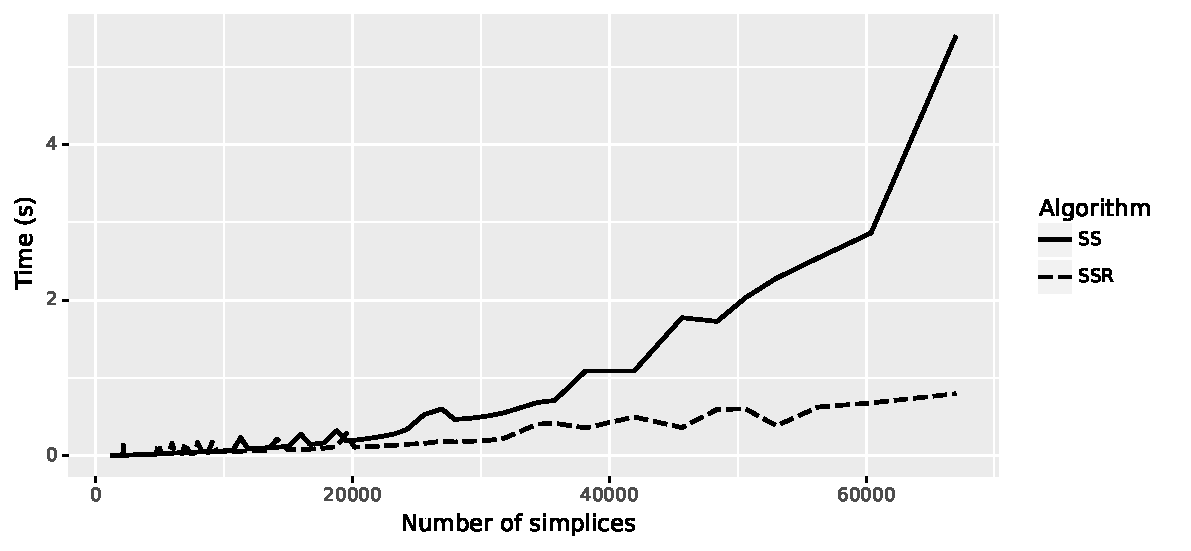
\includegraphics[width=1.2\textwidth]{content/4-comp-top/images/2-2v3-circ-compute}
  }
  \caption{A plot of the running time of \textsc{SS} and \textsc{SSR} algorithms on a Vietoris-Rips complex constructed from a noisy unit circle.}
  \label{fig:speedups-2v3-compute}
\end{figure}

It can be seen that \textsc{SSR} significantly decreases computation time as the number of simplices increase, due to the reduction of column operations. 
